\documentclass{cumcm}
\usepackage{graphicx}
\usepackage{appendix}
\numberwithin{equation}{section}
\numberwithin{equation}{subsection}
\usepackage{csvsimple}
\usepackage{listings}
\usepackage{xcolor}
%\renewcommand{\baselinestretch}{1.0}
%\newcommand{\songtiB}

% \title{text}这里是显示在第三页的文章标题
\title{\textbf{计算机系统结构实验报告\quad 实验4}\\{\Large 简单的类MIPS单周期处理器实现:寄存器、存储器与有符号扩展}}
\author{方泓杰\ 518030910150}


\begin{document}
\maketitle

\begin{abstract}
  本实验实现了简单的类MIPS处理器的几个重要部件:寄存器(Register)、存储器(Data Memory)以及有符号扩展单元(Sign Extension),其作用分别是暂时存放一些数据与运算结果、用于较大量存储数据以及对立即数进行有符号拓展。对于存储部件(如寄存器、存储器等),其需要实现读取数据、存放数据和写入数据的功能。本实验通过软件仿真的形式进行实验结果的验证。
\end{abstract}

\maketitle \tableofcontents
\newpage

\section{实验目的}\label{section1}
本次实验有如下五个实验目的:
\begin{enumerate}
    \item 理解CPU的寄存器、存储器、有符号扩展;
    \item 掌握寄存器(Register)的实现;
    \item 掌握存储器(Data Memory)的实现;
    \item 掌握有符号扩展单元(Sign Extension)的实现;
    \item 使用功能仿真验证功能实现的正确性。
\end{enumerate}

\section{原理分析}\label{section2}

\subsection{寄存器(Register)原理分析}\label{section2.1}

寄存器(Register)的功能是暂时存储一些数据以及中间运算结果,其需要同时支持双通道数据读取、数据写入的功能,主要接口如图 \ref{fig1} 所示。其内部一共有32个寄存器,因此需要5位二进制数作为寄存器的编号来定位到目标寄存器,故三个表示寄存器编号的接口都接收5位二进制数。我们设计的寄存器内存储的数据为32位二进制数,因此所有的数据接口均接收或发送32位二进制数。

\begin{figure}[htbp]
    \centering
    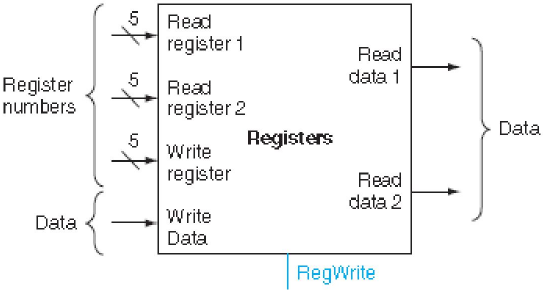
\includegraphics[width=4in]{registers.png}
    \caption{寄存器(Register)的主要接口}
    \label{fig1}
\end{figure}

我们让寄存器的读取数据的操作一直进行,而\underline{写数据的操作仅在时钟下降沿进行}。因为时钟的下降沿处于一个周期的中部,这时候开始写数据可以防止在一个周期开始时读取到错误的数据进而导致的执行结果错误。在后面实验的处理器设计中我们会发现,这个设计至关重要。



\subsection{存储器(Data Memory)原理分析}\label{section2.2}

存储器(Data Memory)的功能是存储大量的数据,其主要包括只读存储器(ROM)以及随机访问存储器(RAM)。我们设计实现的是后者,其需要支持数据读取、数据写入的功能,主要接口如图 \ref{fig2} 所示。在现代的32位计算机中,存储器支持的地址为一个32位二进制数,因此理论上其需要包含 $2^{32}$ 个存储单元;然而由于存在虚拟地址与物理地址的映射,实际上的存储单元数量远小于这个数。\underline{我们在这里不考虑页表、虚拟地址与物理地址的映射,考虑仅含有物理地址的情况}。由于存储大小的限制,我们设计的存储器内部仅能够存储1024个数据,因此理论上只需要10位二进制数即可作为编号,但是我们仍然采用32位二进制数作为编号的方式以尽可能贴近现代计算机的设计;同时,我们\underline{在存储器的内部加入了地址判断的机制},如果给定地址超出了存储器所能够表示的范围 (0到1023),我们就忽略写入操作同时对读取操作返回0。

\begin{figure}[htbp]
    \centering
    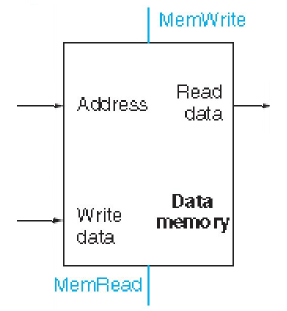
\includegraphics[width=2in]{memory.png}
    \caption{存储器(Data Memory)的主要接口}
    \label{fig2}
\end{figure}

与寄存器类似地,我们让存储器的\underline{写数据的操作仅在时钟下降沿进行}。因为时钟的下降沿处于一个周期的中部,这时候开始写数据可以防止在一个周期开始时读取到错误的数据进而导致的执行结果错误。在后面实验的处理器设计中我们会发现,这个设计至关重要。

\subsection{有符号扩展单元(Sign Extension)原理分析}\label{section2.3}

有符号扩展单元(Sign Extension)的主要功能是将指令中的16位有符号立即数拓展为32位有符号立即数,因此只需要\underline{将这个16位有符号数的符号位填充在32位有符号立即数的高16位},再将低16位复制到32位有符号立即数的低16位即可。我们可以使用Verilog语言提供的拼接操作简单的完成这个功能,具体我们会在第 \ref{section3.3} 节中详细描述。

\section{功能实现}\label{section3}

\subsection{寄存器(Register)功能实现}\label{section3.1}

寄存器(Register)一直进行读取操作,而由RegWrite信号控制是否进行写入操作。在第 \ref{section2.1} 节中我们提到,对于写入操作寄存器将延迟到时钟下降沿时进行写入,这样是为了实现信号同步,同时防止读取到错误数据。而寄存器的读取操作可以一直进行,因为我们会用控制信号来判断读取数据是否为我们需要的数据,而不需要寄存器进行读取数据的检查。

寄存器的部分实现代码如下,完整的代码实现可以参见附录 \ref{appsection1.1}。

\begin{lstlisting}[language=verilog]
reg [31 : 0] regFile [31 : 0];

always @ (readReg1 or readReg2)
begin
    readData1 = regFile[readReg1];
    readData2 = regFile[readReg2];
end
    
always @ (negedge clk)
begin
    if (regWrite)
        regFile[writeReg] = writeData;
end
\end{lstlisting}

\subsection{存储器(Data Memory)功能实现}\label{section3.2}

存储器(Data Memory)由MemRead信号控制是否进行读取操作,而由MemWrite信号控制是否进行写入操作。在第 \ref{section2.2} 节中我们提到,对于写入操作存储器将延迟到时钟下降沿时进行写入,这样是为了实现信号同步,同时防止读取到错误数据。同时在第 \ref{section2.2} 节中我们提到,需要加入对存储器的地址进行检查的机制,以防止写入不存在的存储单元。

存储器的部分实现代码如下,完整的代码实现可以参见附录 \ref{appsection1.2}。
\begin{lstlisting}[language=verilog]
reg [31 : 0] memFile [0 : 1023];

always @ (memRead or address)
begin
    // check if the address is valid
    if (memRead)
    begin
        if(address <= 1023)
            readData = memFile[address];
        else
            readData = 0;
    end
end
    
always @ (negedge clk)
begin
    if (memWrite && address <= 1023)
        memFile[address] = writeData;
end
\end{lstlisting}

\subsection{有符号扩展单元(Sign Extension)功能实现}\label{section3.3}

有符号扩展单元(Sign Extension)将16位有符号立即数扩展为32位有符号立即数。在第 \ref{section2.3} 节中我们提到,将指令中的16位有符号立即数拓展为32位有符号立即数,只需要将这个16位有符号数的符号位填充在32位有符号立即数的高16位,再将低16位复制到32位有符号立即数的低16位即可。我们这里使用Verilog提供的拼接操作,将16为有符号数的符号位复制16份,与原数拼接后得到符号扩展后的结果。

有符号扩展单元的部分实现代码如下,完整的实现代码可以参见附录 \ref{appsection1.3}。

\begin{lstlisting}[language=verilog]
assign data = { {16 {inst[15]}}, inst[15 : 0] };
\end{lstlisting}


\section{结果验证}\label{section4}

\subsection{寄存器(Register)结果验证}\label{section4.1}

我们使用Verilog编写激励文件,采用软件仿真的形式对寄存器(Register)模块进行测试(代码实现参见附录 \ref{appsection2.1})。我们在激励文件中对寄存器读写的不同情况进行了测试,测试结果如图 \ref{fig3} 所示。

\begin{figure}[htbp]
    \centering
    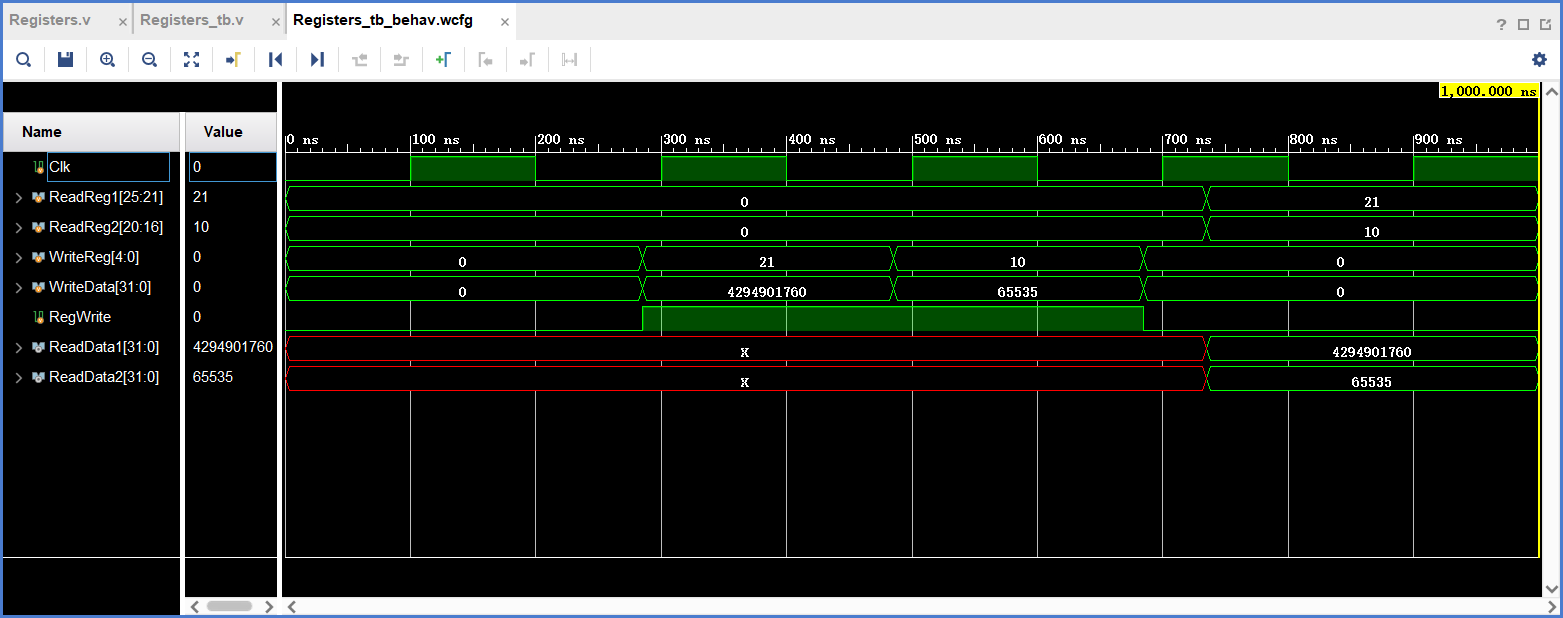
\includegraphics[width=6.3in]{1.png}
    \caption{对于寄存器(Register)的测试结果}
    \label{fig3}
\end{figure}

注意我们的测试结果和实验指导书上的测试结果略有不同,我们的readData接口的前面一段数据为 \texttt{x},\underline{这是由于寄存器数据没有进行初始化}。\textbf{由于本次实验没有初始化要求,因此询问老师后我们得知这种结果也是正确的}。同时,关于寄存器的其他操作的执行结果都是正确的,因此寄存器的仿真成功,说明寄存器实现正确。

\subsection{存储器(Data Memory)结果验证}\label{section4.2}

我们使用Verilog编写激励文件,采用软件仿真的形式对存储器(Data Memory)模块进行测试(代码实现参见附录 \ref{appsection2.2})。我们在激励文件中对存储器读写的不同情况(甚至包含了同时读写的特殊情况)进行了测试,测试结果如图 \ref{fig4} 所示。

\begin{figure}[htbp]
    \centering
    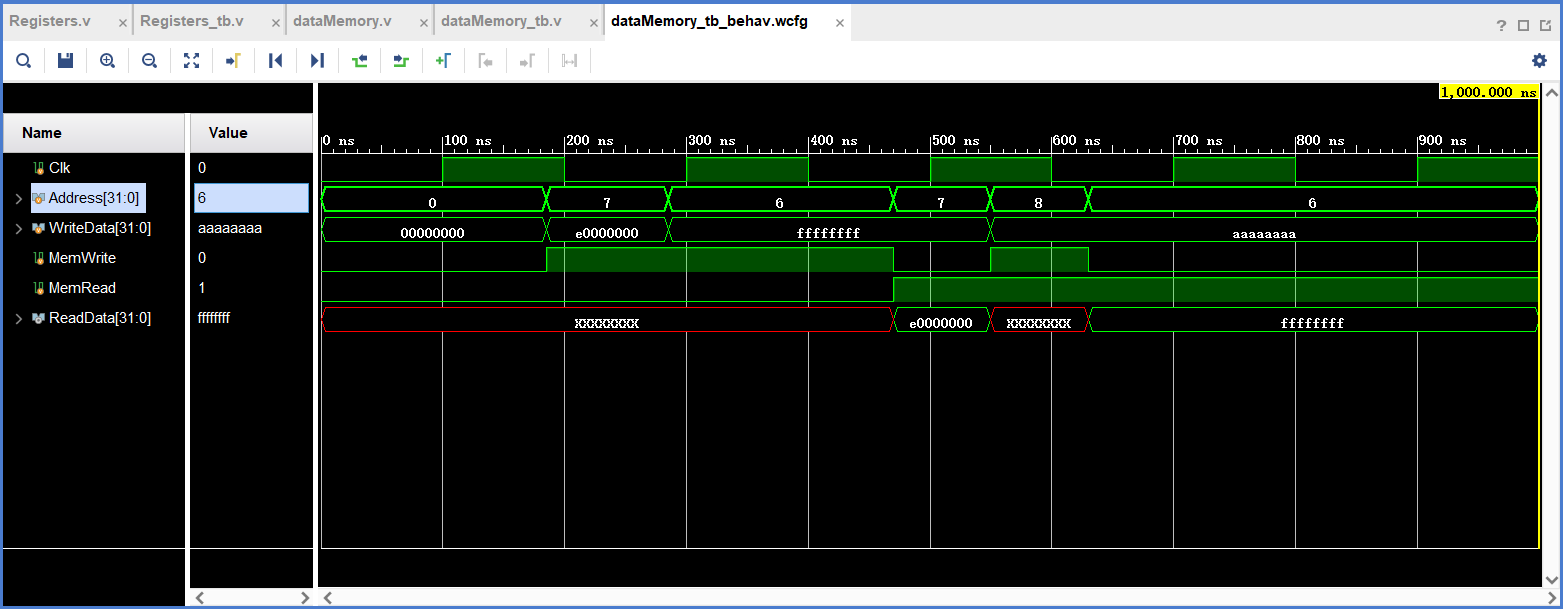
\includegraphics[width=6.3in]{2.png}
    \caption{对于存储器(Data Memory)的测试结果}
    \label{fig4}
\end{figure}

注意我们的测试结果和实验指导书上的测试结果略有不同,我们的readData接口的前面一段数据为 \texttt{x},\underline{这是由于存储器数据没有进行初始化}。同时,我们readData接口中间的一段数据也是 \texttt{x},\underline{这是由于我们将写操作延迟到时钟下降沿},从而导致读操作执行时,其读到的数据没有进行初始化。\textbf{询问老师后,我们得知这种结果也是合理的}。同时,关于存储器的其他操作的执行结果都是正确的,因此存储器的仿真成功,说明存储器实现正确。


\subsection{有符号扩展单元(Sign Extension)结果验证}\label{section4.3}

我们使用Verilog编写激励文件,采用软件仿真的形式对有符号扩展单元(Sign Extension)模块进行测试(代码实现参见附录 \ref{appsection2.3})。我们在激励文件中对有符号扩展单元的不同输入都进行了测试,测试结果如图 \ref{fig5} 所示。

\begin{figure}[htbp]
    \centering
    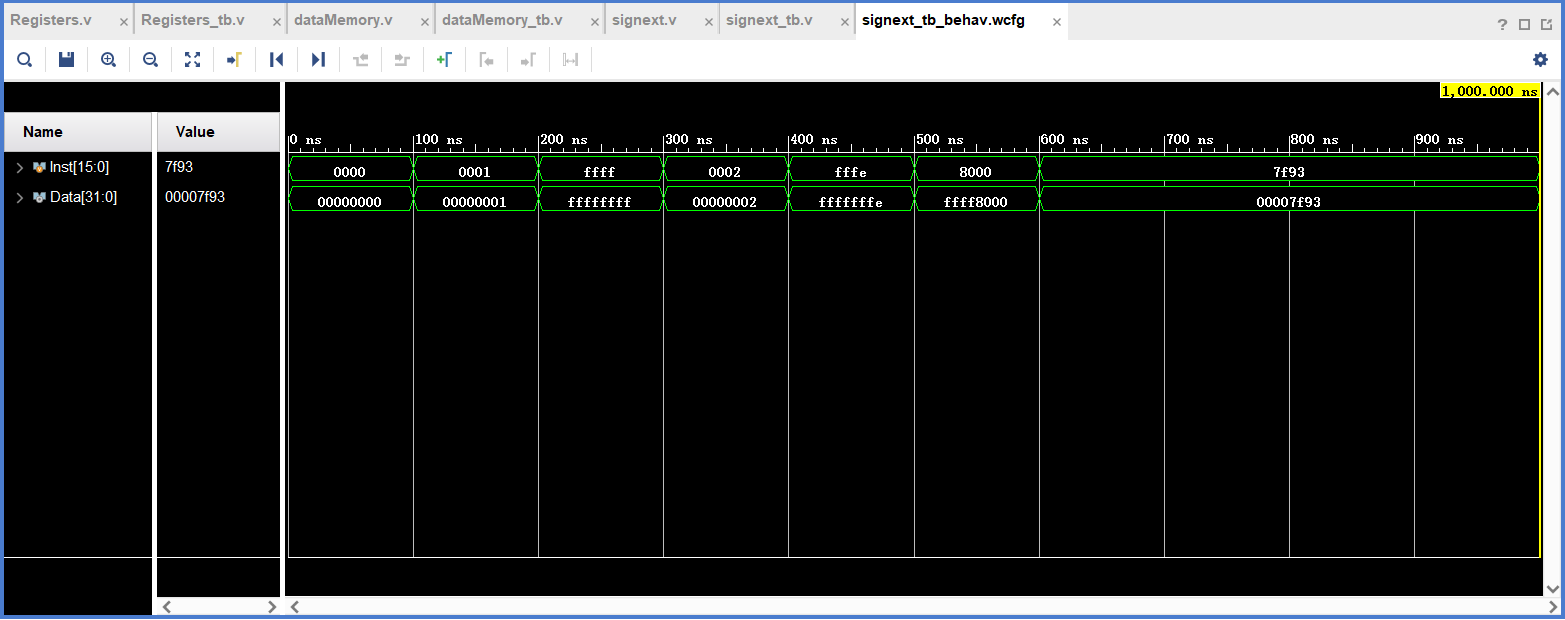
\includegraphics[width=6.3in]{3.png}
    \caption{对于有符号扩展单元(Sign Extension)的测试结果}
    \label{fig5}
\end{figure}

可以发现,有符号扩展单元正确扩展了每个输入数据,因此仿真成功,有符号扩展单元实现正确。

\section{总结与反思}\label{section5}
本实验设计并实现了类MIPS处理器的三个重要组成部件:寄存器(Register)、存储器(Data Memory)、有符号扩展单元(Sign Extension),并且通过软件仿真模拟的方法验证了它们的正确性,为后面的单周期类MIPS处理器以及流水线处理器的实现奠定基础。同时,这也运用了我在第二次实验的报告中所提到的“子元件”的思想,这种思想可以将一个较为复杂的电路(如整个处理器)拆分成许多功能简单、易于实现的元件进行实现(如本次实验中实现的三个小元件)。

同时,本次实验还较为基础,没有考虑到一些特殊指令对于元件的要求(如jal指令可能需要寄存器开辟新的接口用于快速跳转等等);在后续的实验中,我们将对本次实验设计的几个模块进行逐步的完善,加入一些实现的细节来更好组装整个处理器。

在本次实验的过程中,我发现了寄存器与存储器的仿真结果与实验指导书上的结果略有不同,经过分析后发现这种不同是由于初始化以及延迟写操作等原因共同导致,与老师进行讨论后发现,寄存器与存储器的实现本身没有问题。这个经历锻炼了我分析处理问题的能力。

本次实验的一个重要思想是:延迟存储器、寄存器的写操作到时间下降沿。这样可以同步信号,保证读取数据的正确性,保证程序运行正确,这是一个非常重要的设计理念,值得深入研究。总之,本次实验让我对这三个部件有了更加深入的认识。


\section{致谢}\label{section6}
感谢本次实验中指导老师在课程微信群里为同学们答疑解惑;

感谢上海交通大学网络信息中心提供的远程桌面资源;

感谢计算机科学与工程系相关老师对于课程指导书的编写以及对于课程的设计,让我们可以更快更好地学习相关知识,掌握相关技能;

感谢电子信息与电气工程学院提供的优秀的课程资源。
%\bibliographystyle{plain}
%\bibliography{ref}

\clearpage
\begin{appendices}
\section{设计文件完整代码实现}\label{appsection1}
\subsection{寄存器(Register)的代码实现}\label{appsection1.1}
参见代码文件 \texttt{Registers.v}。
\subsection{存储器(Data Memory)的代码实现}\label{appsection1.2}
参见代码文件 \texttt{dataMemory.v}。
\subsection{有符号扩展单元(Sign Extension)的代码实现}\label{appsection1.3}
参见代码文件 \texttt{signext.v}。
\section{激励文件完整代码实现}\label{appsection2}
\subsection{寄存器(Register)激励文件的代码实现}\label{appsection2.1}
参见代码文件 \texttt{Registers\_tb.v}。
\subsection{存储器(Data Memory)激励文件的代码实现}\label{appsection2.2}
参见代码文件 \texttt{dataMemory\_tb.v}。
\subsection{有符号扩展单元(Sign Extension)激励文件的代码实现}\label{appsection2.3}
参见代码文件 \texttt{signext\_tb.v}。
\end{appendices}

\end{document}
